\chapter{Future Work and Conclusion}

With the number of data sources and sensors networks increasing in the world, context discovery has a very exciting and promising future. More importantly, with the increase in sources, it will become extremely important to be selective about what information to consider context and what not. In this dissertation, we presented a context based technique to prune the search space for the entity identification problem in multimedia objects, specifically personal photos. We used a relation centric perspective of contextual information to progressively discover context which is relevant to a given photo. In the cases where only partial context is available, we saw how propagation techniques can help us order persons by propagating context from nearby photos and other events.


\section{Future Work}
The techniques described in this dissertation present a number of future opportunities. Here we list some of the open problems faced by context discovery techniques in general and some extensions to the algorithms described in the previous chapters. 

\begin{enumerate}
  \item The notion of relevance in context is currently specific to our application. Creating a generic notion, backed by mathematical infrastructure is an open problem. Since we are relating propagation techniques to context discovery, it might be possible to extend and relate some of the theoretical literature developed for random walks in graphs to events and time based context discovery. Any formulation of bounds in the sizes or growth rates of context network would result in very important implications of future algorithms.

  \item All the data structures and algorithms described in the previous chapters cater to tagging few number of photos at a time. Performing the same work on a very large scale (billions of photos), is an open problem. It is also not clear if existing large scale computational infrastructures like Map Reduce or Pregel are an efficient foundation to perform context discovery.

  \item In our work, we assume the correctness of context obtained from different sources. In the real world, this might not be so. Some context might be fake or some might just be incorrect. In order to deal with such cases, backtracking to a previously constructed accurate context network might become an important step in the discovery process. What data structures allow such an operation (in our case, we have no way of saying which nodes were merged in which previous stage) correctly, efficiently and in a scalable manner is not known.

  \item The real world is very complicated. There are many entities which can influence each other, and in many different ways. Specifying real world knowledge has been one of the hardest problem faced by computer scientists for decades. OWL ontologies although meritorious in their own right, were designed to solve the data integration problem. It is cumbersome to describe many aspects of the real world knowledge using OWL, some of which is contradicting and contains exceptions. For example consider the piece of knowledge: bacteria \textit{Bacillus Subtilis} is a catalyst to rock weathering. So large quantities of this bacteria can lead to severe rock weathering, which is usually accompanied by carbon dioxide consumption. By reducing carbon dioxide in the atmosphere can lead to reduction in overall temperature. The bacteria can only exist in parts of the world with favorable weather (an assertion on atmospheric temperature value). Notice the cycle of causation here. It is non trivial to model and reason with such knowledge which is very common in many domains and is crucial for this technology to be improved or engineered before advancing CueNet to such domains.

\end{enumerate}

\section{Applications}
Besides identifying entities in multimedia objects, CueNet can be utilized in a variety of other applications. We identify some of the brave new world applications, and describe them below:

\begin{enumerate}
  \item \textbf{Contextual Narratives}: Multimodal stories are rich in context. Almost all social networks and public news feeds are overloaded with noise. There is so much content, and so little context, that the situation demands active attention from users to sift through the data to put information into context. With context discovery, models about real world events and heterogeneous information about entities from various sources can be combined and summarized to produce coarse or fine grained narratives about important public or personal events. Of course, there is sometimes no better substitute than adding a narrator in the loop to improve the final quality of such stories. In such a case, context discovery will have to be modified to work in synergy with humans for better results.

  \item \textbf{Disease Identification}: Studying the symptoms of a patient and coming up with a medical diagnosis is a very hard problem. Given the increasing number of medical sensors and personal health applications, it is becoming increasingly easy to construct a `full body scan kit right at home'. With large amounts of computational power becoming available, and using the large number of tests available from their literature, a version of CueNet can be tailor made to diagnose people who are showing signs of weakening health. Instead of verifying faces, this system would be conducting specific medical tests (such as blood sugar sampling, WBC count or temperature check) in conjunction with analyzing with what the person ate, where he traveled or with whom he spent time (and if any of these people had shown such symptoms). Progressively, the system will discover which parts of the body are infected, and proceed to raise appropriate warning, along with presenting detailed reports on the infection's origin, expected symptoms over the next few days and preventive measures.

  \item \textbf{Situation-Based Advertising}: Advertising on the web is largely driven by content on the web or textual results from search engines. Thus, many people see ads which are irrelevant at that time. But with context discovery, context networks can be matched for specific patterns which can lead to more precise ``needed-at-that-time" pattern. For example, suppose a person comes to know that a friend met with a skateboarding accident and is at the nearby hospital. The system can check this friend's wishlist on Amazon and find that it contains the new album by some of his favorite bands, which is available on a shop which is halfway between the friend and the person. The system can also check if any of these shops have signed copies of the records making the gift more meaningful.


\end{enumerate}

\section{Known Issues}
In this section, we list some of the issues encountered in designing and building CueNet. Some of these are active areas of research, and whereas others are specific to our framework, and can be considered potential areas of research. Our experience with CueNet indicates that the following issues should be approached in a holistic manner, i.e., in conjunction with each other. Approaching these problems in the context of each other reduces the individual complexity of each sub-problem by possibly increasing the complexity of the entire framework, but making the problem more tractable.

\textbf{\textbf{Noise in Social Media}}: The problem of noise filtering in web data is a prominent one, and is being addressed by various communities in different ways. These range from entity matching and record linkage problems \cite{elmagarmid2007duplicate} to correcting missing data in information networks \cite{sadikov2011correcting}. These problems get trickier because of the different variations in representing tiny details such as representation names of people, addresses of places, and time. In fact, there is a whole school of anthroponomastics \cite{schneider2009s} dedicated to studying variations in human names. Ideas in this field indicate that these differences arise due to cultural, historical and environmental issues\cite{al2009socio}. Such issues cannot be trivially addressed. Consider, for example, the Hebrew name below:

\begin{figure}[h]
\centering
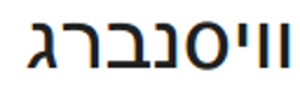
\includegraphics[width=0.5\textwidth]{media/ronen.png}
\label{fig:exp-general-loc-cx}
\end{figure}

It can be translated to English as ``Waisenberg" or ``Vaisenberg". So are Mr.\ X Waisenberg who authored a paper in a Security conference and Dr.\ X Vaisenberg who works at Google, the same person? They might be if X has semitic origins!

Face tags in social media sources like Facebook can also be very noisy. This strictly prohibits directly using this data to train verification/recognition models. Also, the quality of photos are poor, resulting in weaker features, which would have otherwise allowed better matching. 

An exhaustive scientific characterization of noise in social media is beyond the scope of this dissertation, and is being investigated step by step in social media research communities.

\textbf{\textbf{CPU Efficiency}}: The query engine in CueNet is responsible for extracting data from different sources. If a very large number of photos are being tagged, our scheme of query generation and merging will prove inefficient. Processing many photos from different people provides a very rich opportunity to develop interesting heuristics using event semantics for the multi-query optimization problem. Also, partitioning the discovery algorithm such that the computations can occur in a distributed manner is a complex problem. Such steps will be required if the application workload is of the scales of Facebook or processing photos in real time at the scales of Instagram.

\textbf{\textbf{Face Verification}}: Even though face recognition has been studied in research for the last two decades, face verification, and its specific application to faces in the wild has been a relatively recent venture. Although the accuracy of these systems is commendable, the problems of occlusion, image quality, face alignment and differing lighting conditions exist. These hard problems need to be solved before ``perfect" or ``near-perfect" verification can be established. 

\textbf{\textbf{Execution Patterns}}: When is a good time to execute the algorithm? When a user takes a photo? Or before she uploads it to her favorite photo sharing site? For the current evaluation, contextual sources are assumed to be immutable. This is not true in the real world. Contextual sources are constantly being appended with new information, and old information is being updated. These updates may be vital in tagging a certain photo. So the question of when to execute the algorithm, or how and when to query the sources is an open question. If a large number of photos are to be tagged, and a busy source like Facebook is being used for context, the CueNet query engine must take into account various freshness metrics and crawling policies of the sources. 

\textbf{\textbf{Open Datasets}}: The unavailability of a large public data set over which different techniques can be evaluated against each other is an open problem. As seen in our experiments, personal information is vital to contextual approaches, and this data is largely personal, and therefore cannot be shared openly. Optimal anonymization techniques need be to invented such that the privacy of the experiment participants are maintained, and at the same time the data is meaningful to be applied in contextual approaches to problems. This need to be solved so that new context discovery techniques can be evaluated independently and against each other, over a common platform.

In short, we have introduced the challenging, yet fascinating, problem of context discovery. Which becomes harder when considering scaling issues. Which becomes even harder when considering domains which are more detailed and complex than face tagging in photos. But a problem which is inevitable, and must be tackled to improve many aspects of human society and push it to the next frontiers. To put it in words which every science fiction geek has heard before:

\centering
To boldly go where no man has ever gone before \\
\setlength{\parindent}{8cm} \texttt{ Star Trek (1966 - ) } 